\section{Architecture of the System}
\phantomsection
\subsection{UML Diagrams}
The Unified Modeling Language (UML) is a development and all use modeling language in the field of software engineering. Is indended to assure a standard way of visualizing the design of the system that it was made for.
To describe Kyno, the following UML diagrams will be used
\begin{itemize}
\item Use Case Diagram;
\item Deployment Diagram;
\item Class Diagram
\item Sequence Diagram;
\item Activity Diagram;
\item State Diagram.

\end{itemize}
These diagrams will illustrate the users possibilities, the system architecture and will also illustrate the procedures of interaction between the modules.

\subsubsection{Use Case Diagram}

\begin{figure}[!h]
\centering
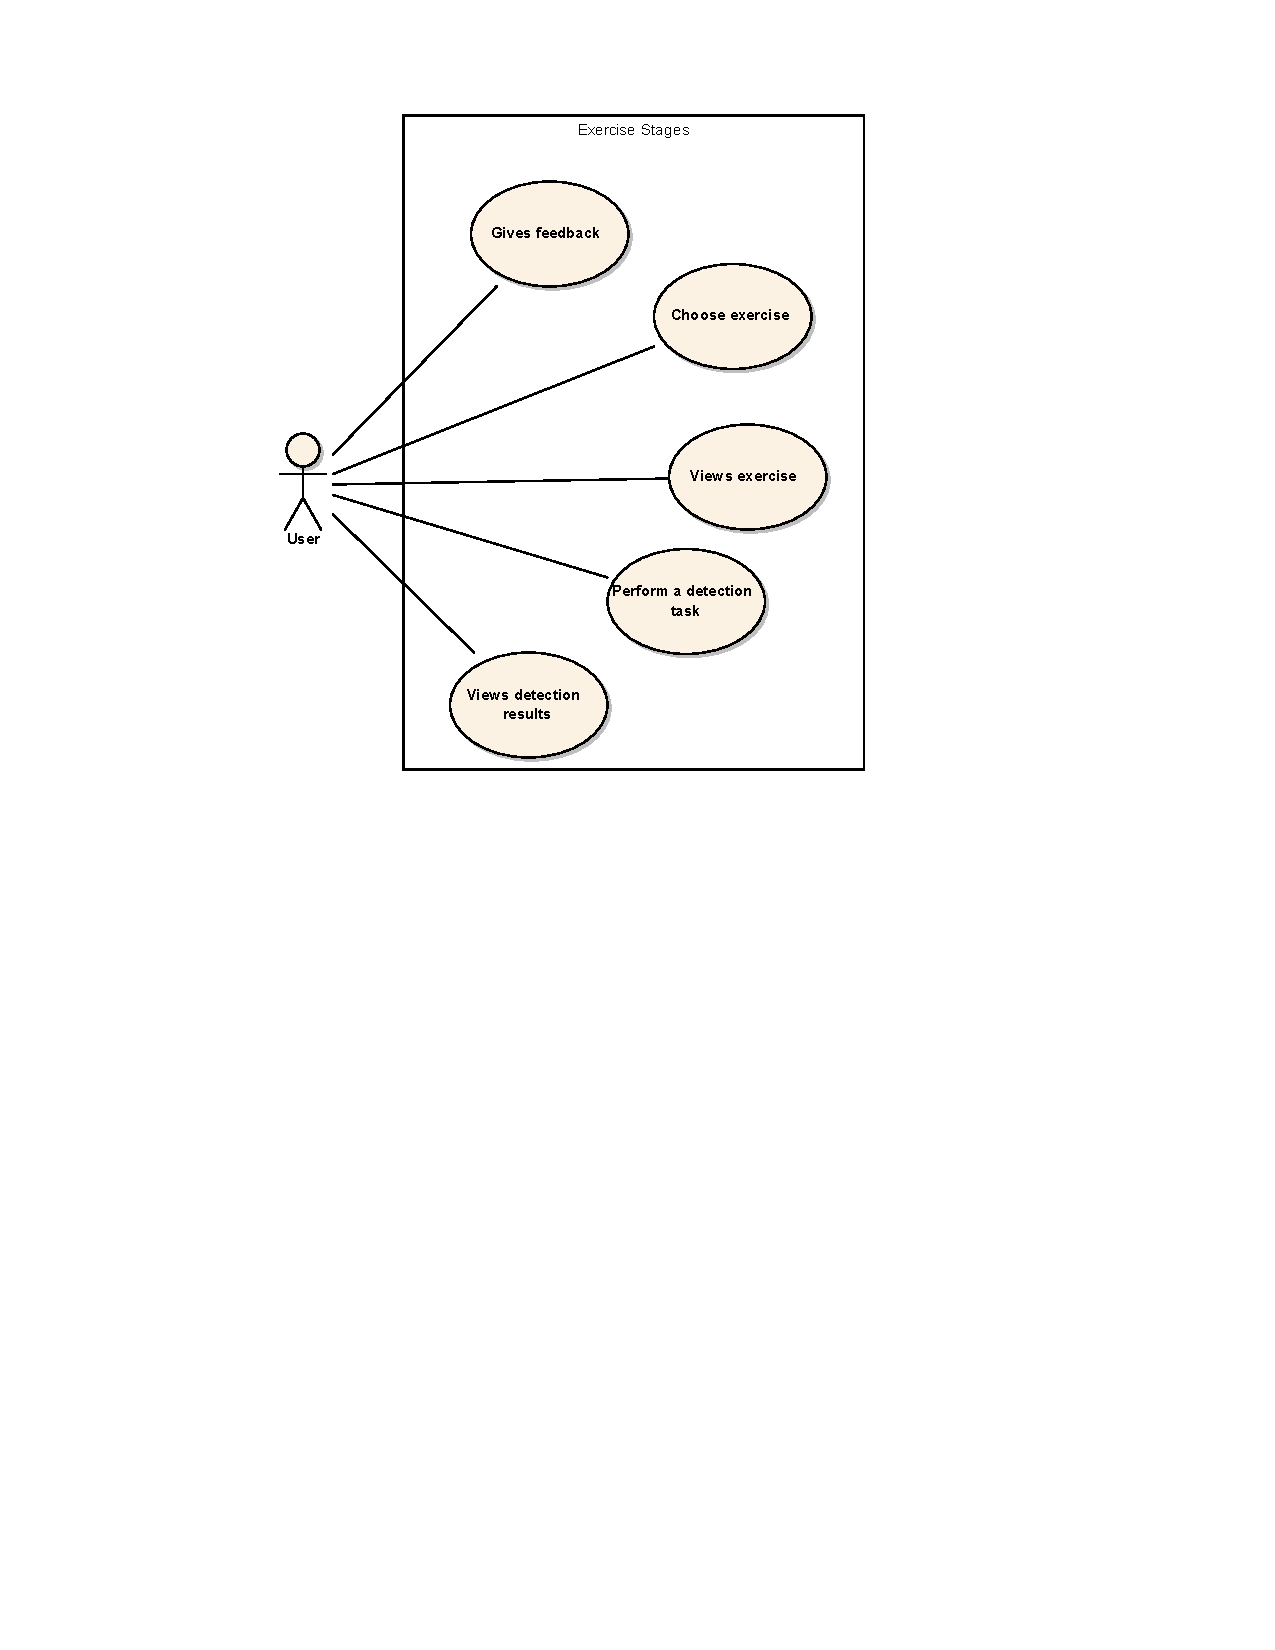
\includegraphics[trim={0 14.5cm 0 1cm},clip, width = 16cm]{2_uc_general}
\caption{General Use Case diagram of the system.}\label{uc_general}
\end{figure}

\begin{figure}[!h]
\centering
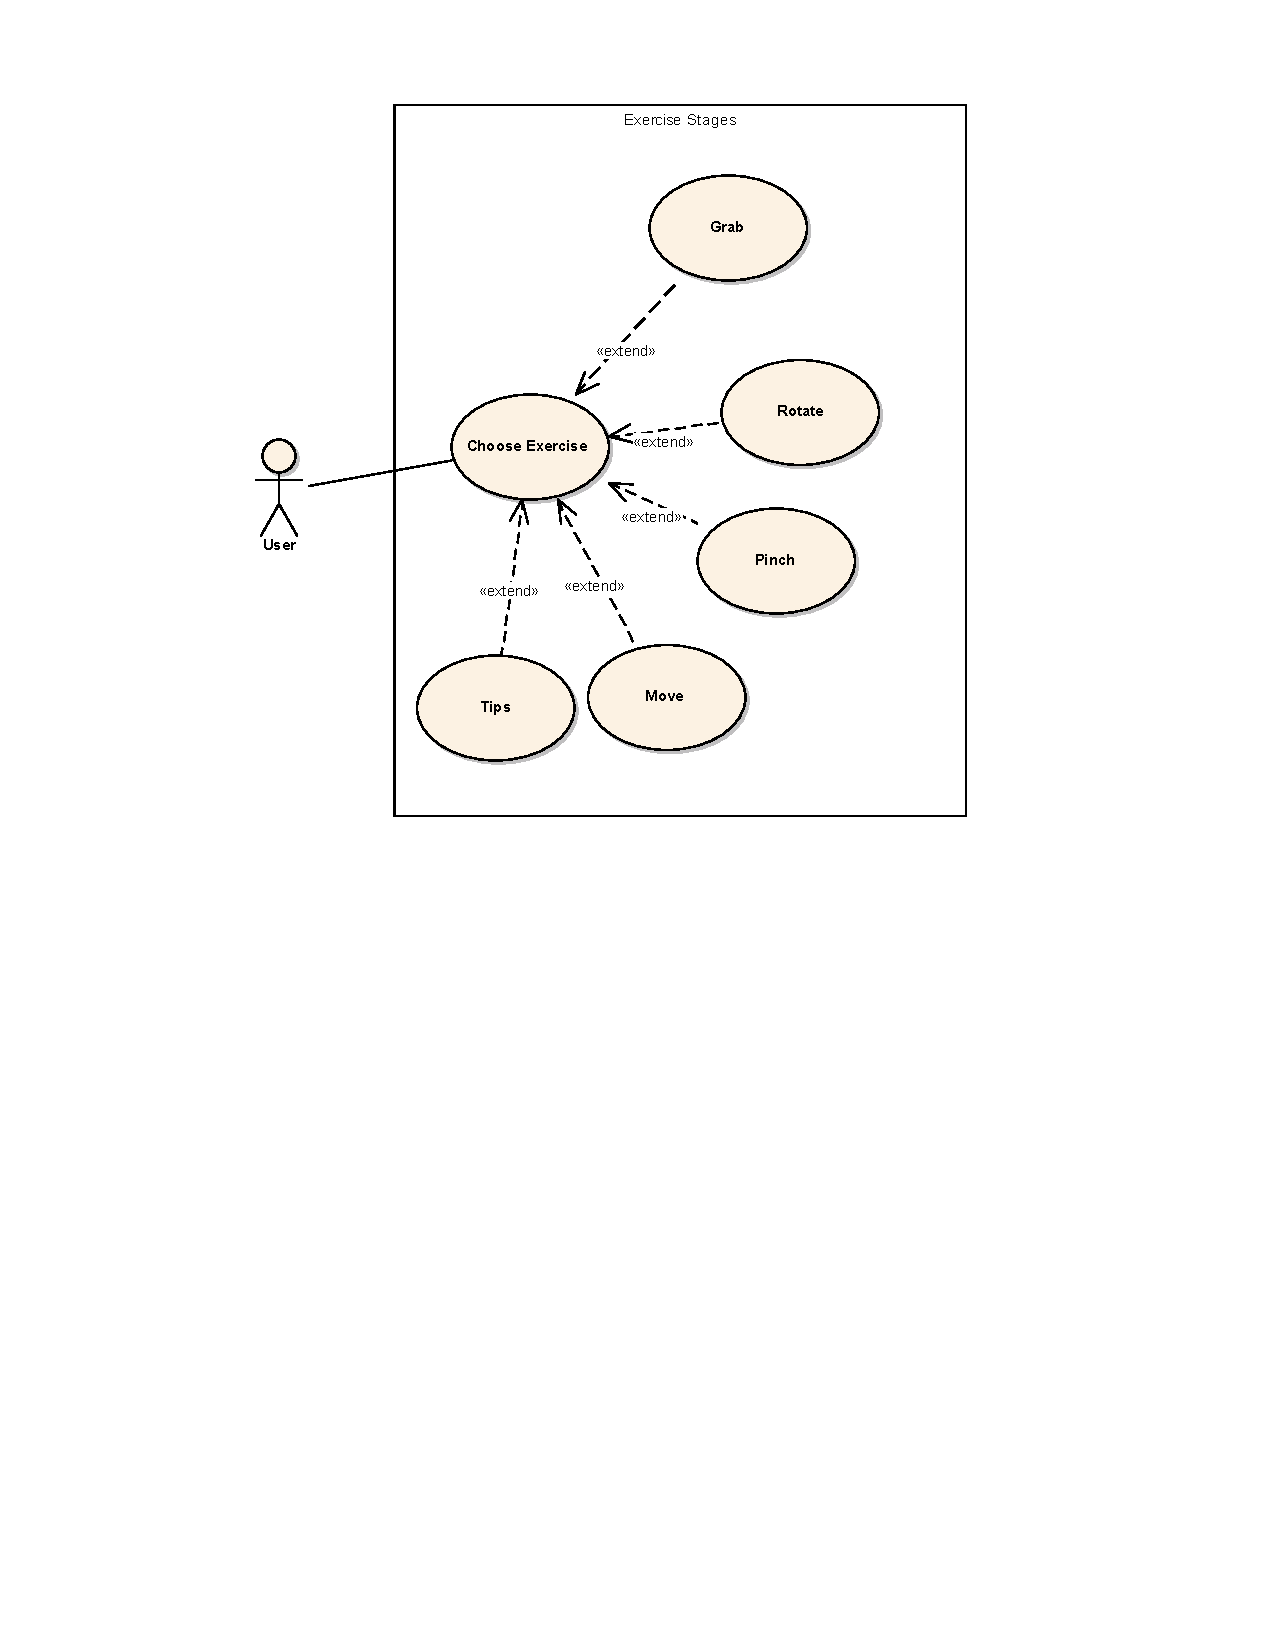
\includegraphics[trim={0 14cm 0 1cm},clip, width = 16cm]{1_uc_exercise_stage}
\caption{Use Case diagram of exercise steps.}\label{uc_exercise}
\end{figure}

\clearpage
\subsubsection{Deployment Diagram}

\begin{figure}[!h]
\centering
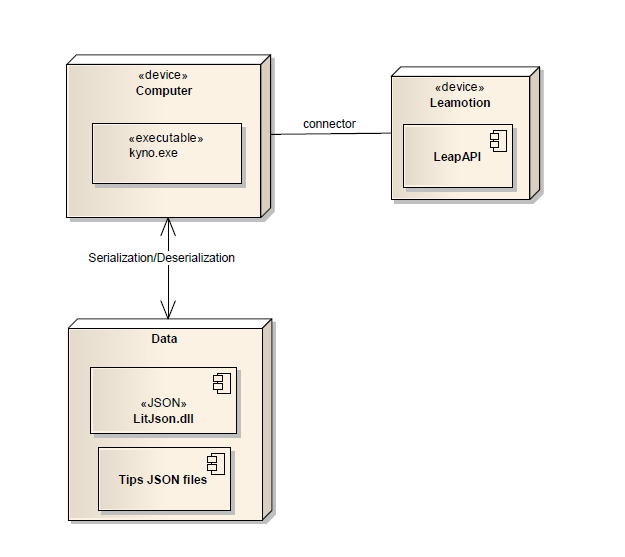
\includegraphics[trim={0 15.5cm 0 2cm},clip, width = 16cm]{1_deploy_diagram}
\caption{Deploy diagram of the system.}\label{deploy_diagram}
\end{figure}

\clearpage

\subsubsection{Class Diagram}
\begin{figure}[!h]
\centering
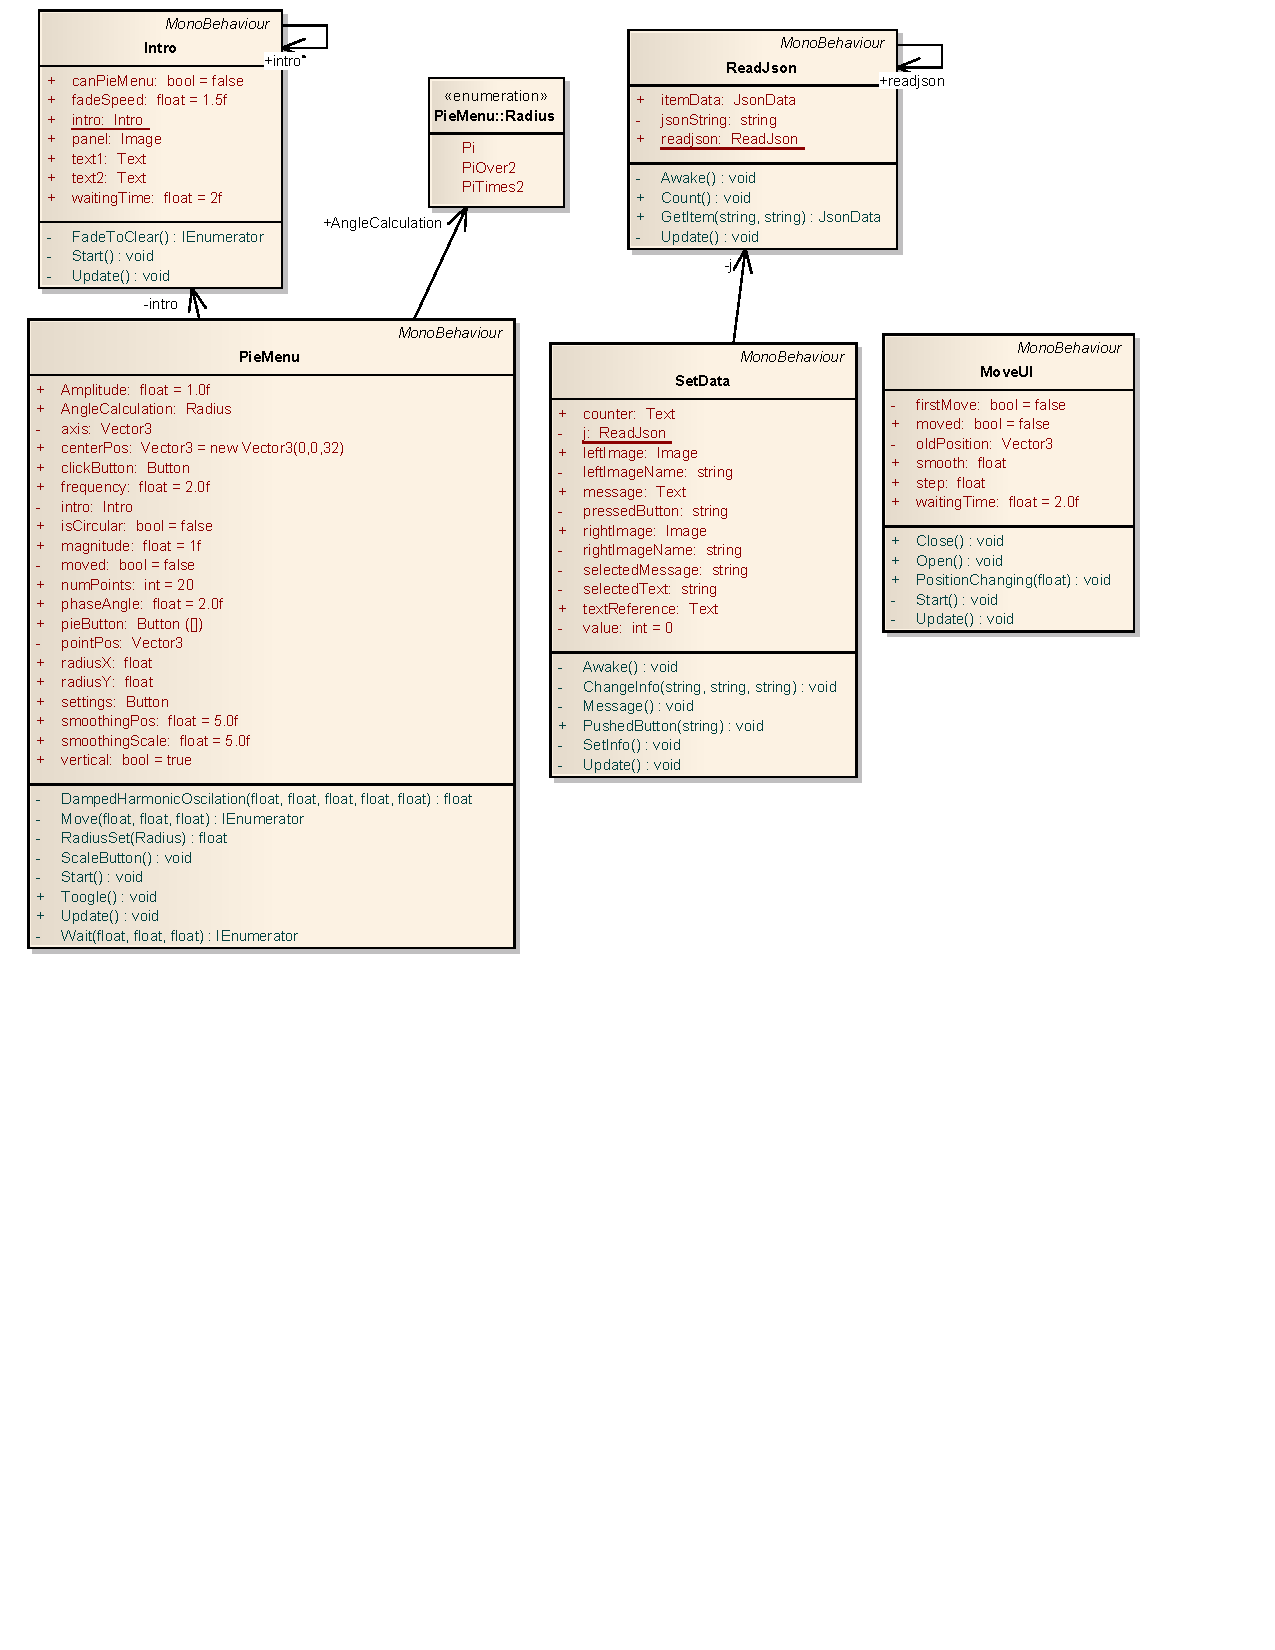
\includegraphics[trim={0 11cm 0 0cm},clip, width=16cm]{1_class_ui}
\caption{Class Diagram of User Interface and User Interaction.}\label{class_ui}
\end{figure}

\clearpage

\begin{figure}[!h]
\centering
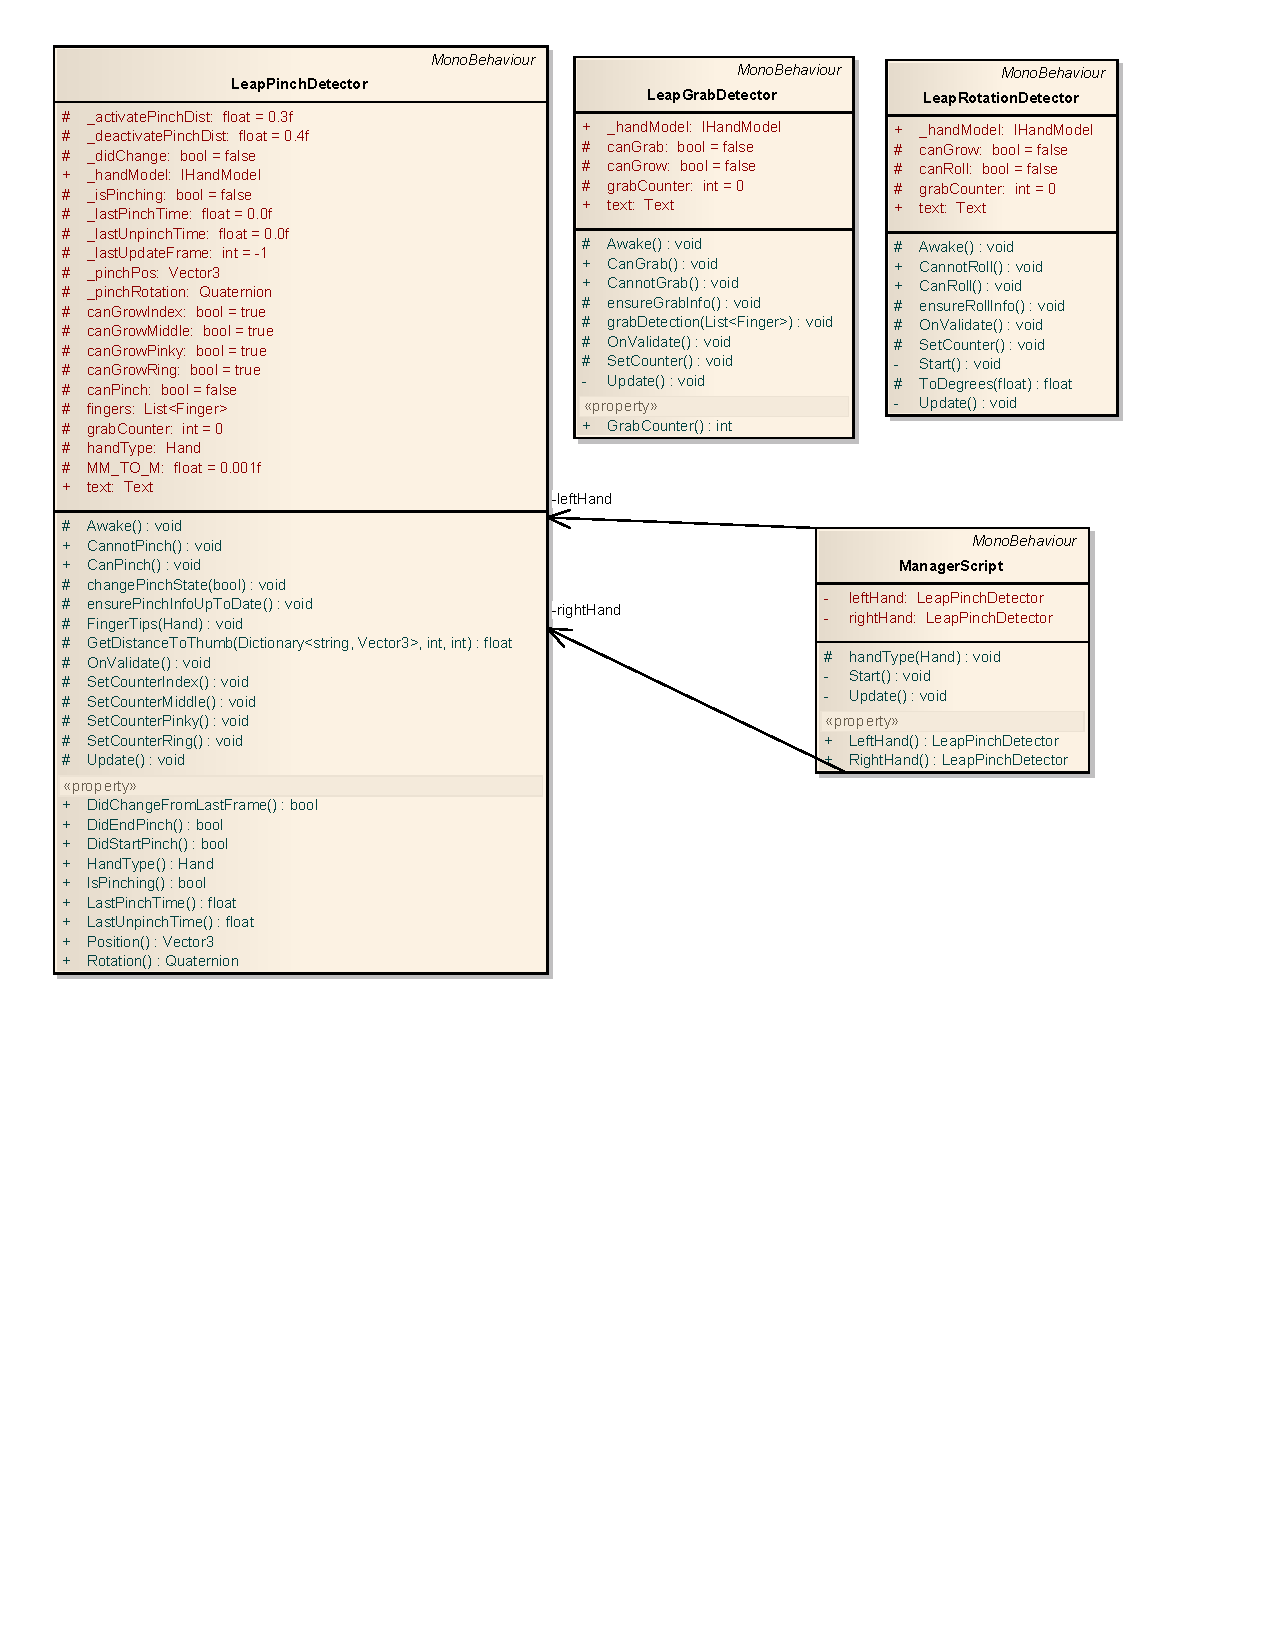
\includegraphics[trim={0 11cm 0 0.5cm},clip, width=16cm]{2_class_leapstates}
\caption{Class Diagram of Leap Motion gesture tracking.}\label{class_leap}
\end{figure}

\clearpage

\subsubsection{Sequence Diagram}
\begin{figure}[!h]
\centering
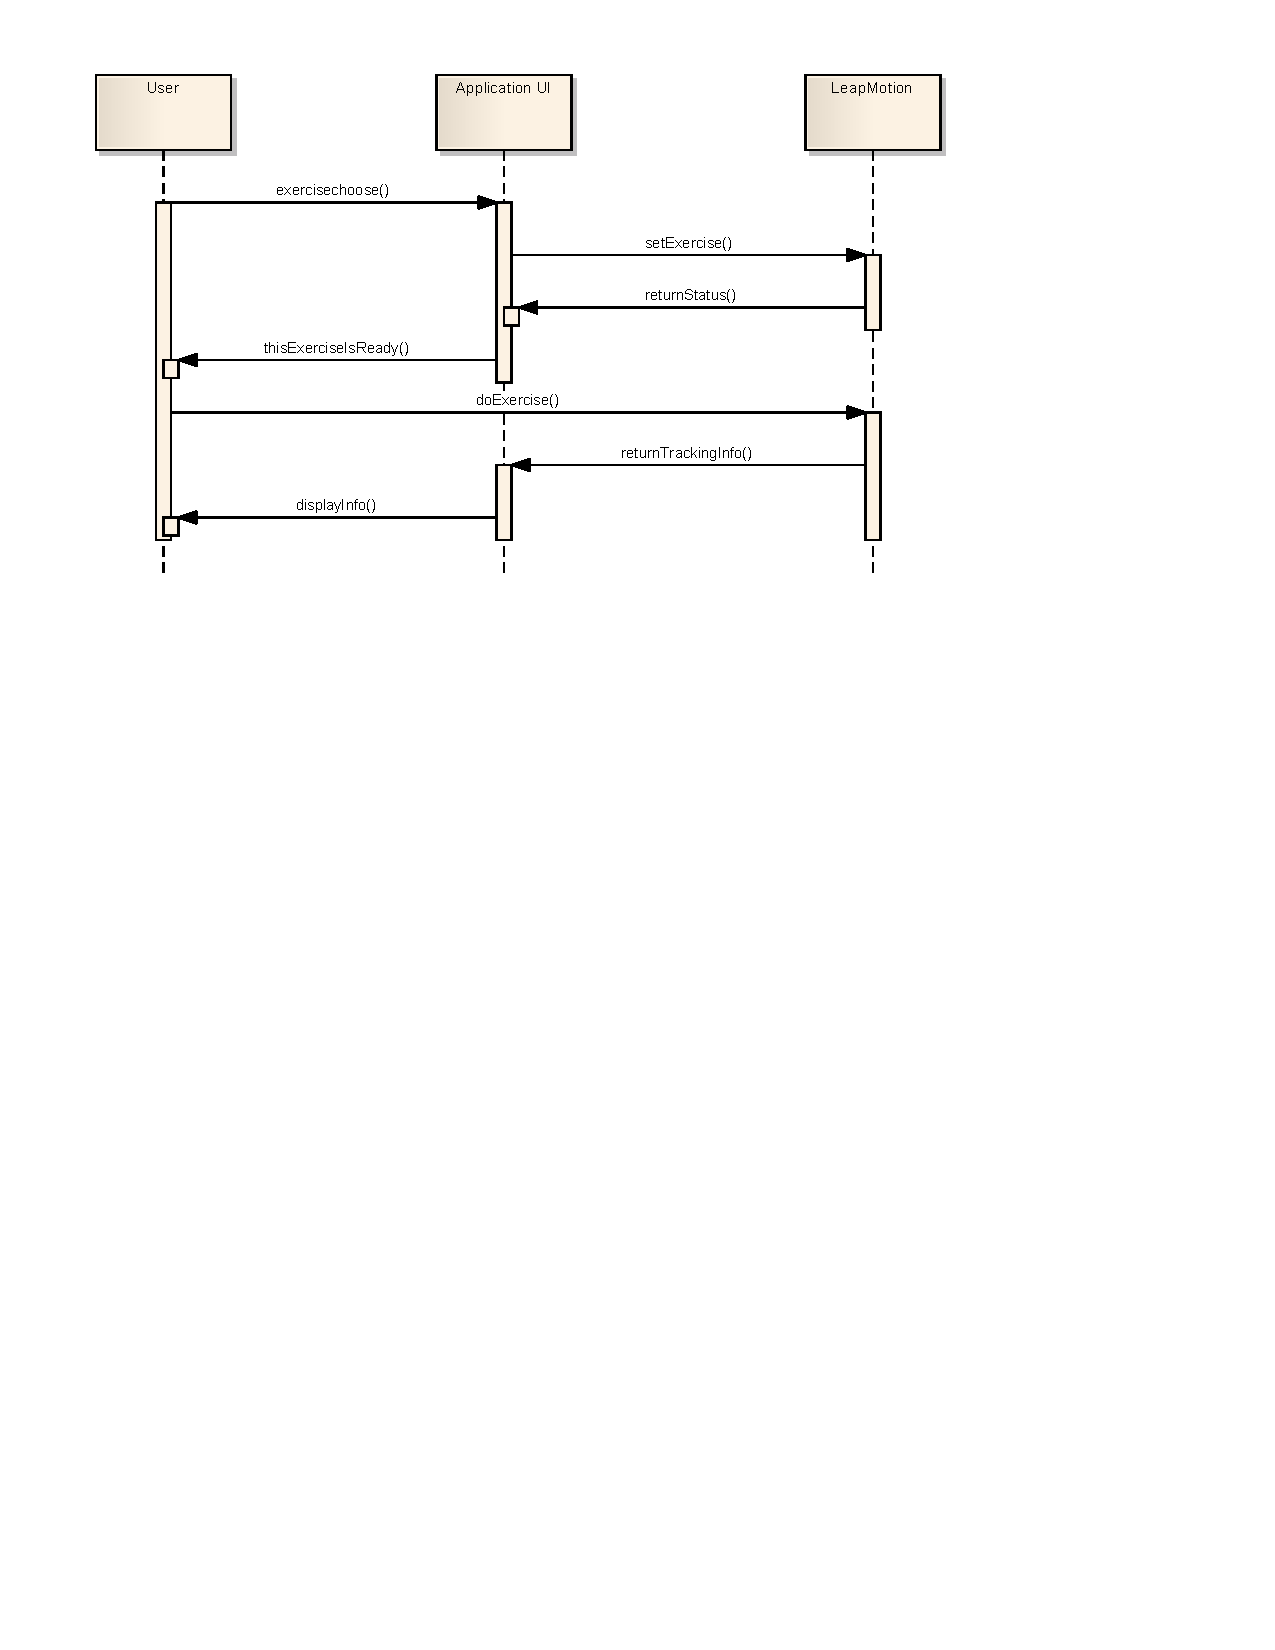
\includegraphics[trim={0 18cm 0 1cm},clip, width = 16cm]{1_sequence_exercise}
\caption{Sequence diagram of doing an exercise set.}\label{sequence_exercise}
\end{figure}

\clearpage

\subsubsection{Activity Diagram}
\begin{figure}[!h]
\centering
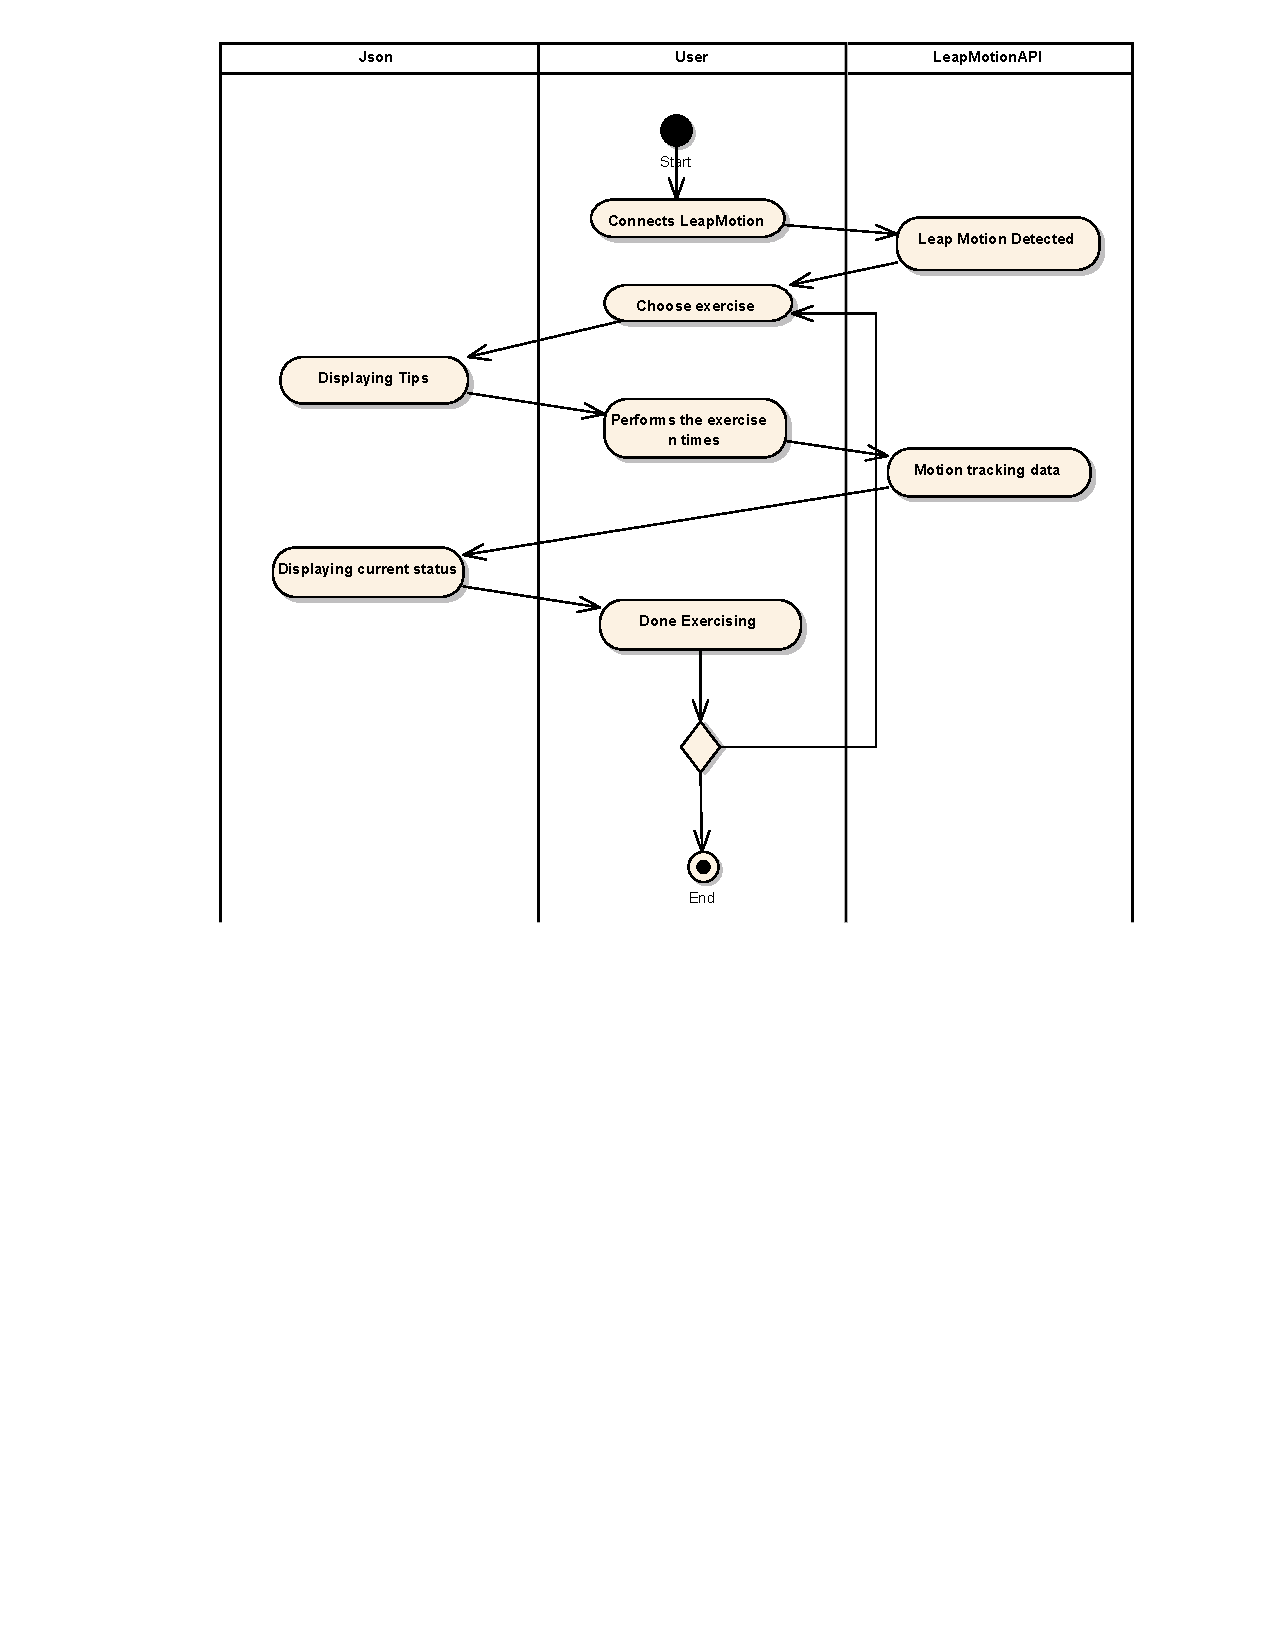
\includegraphics[trim={2cm 14cm 0 0.5cm},clip, width = 16cm]{1_activity_performs_exercise}
\caption{Activity diagram of performing an exercise.}\label{activity_performs}
\end{figure}1

\clearpage

\subsubsection{State Diagram}

\begin{figure}[!h]
\centering
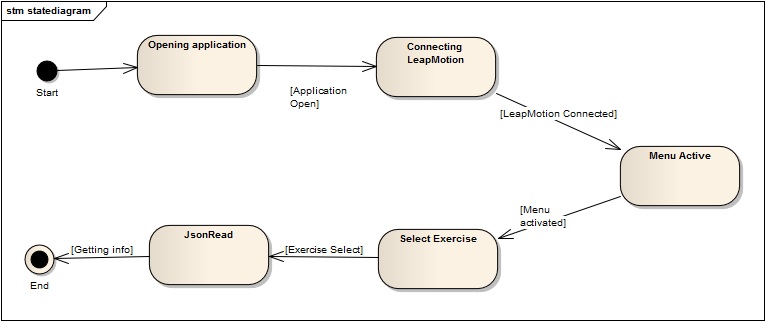
\includegraphics[trim={0 18cm 0 2cm},clip, width = 16cm]{1_state_chooseExercise}
\caption{Activity diagram of choosing and exercise.}\label{state_choose}
\end{figure}

\clearpage

\begin{figure}[!h]
\centering
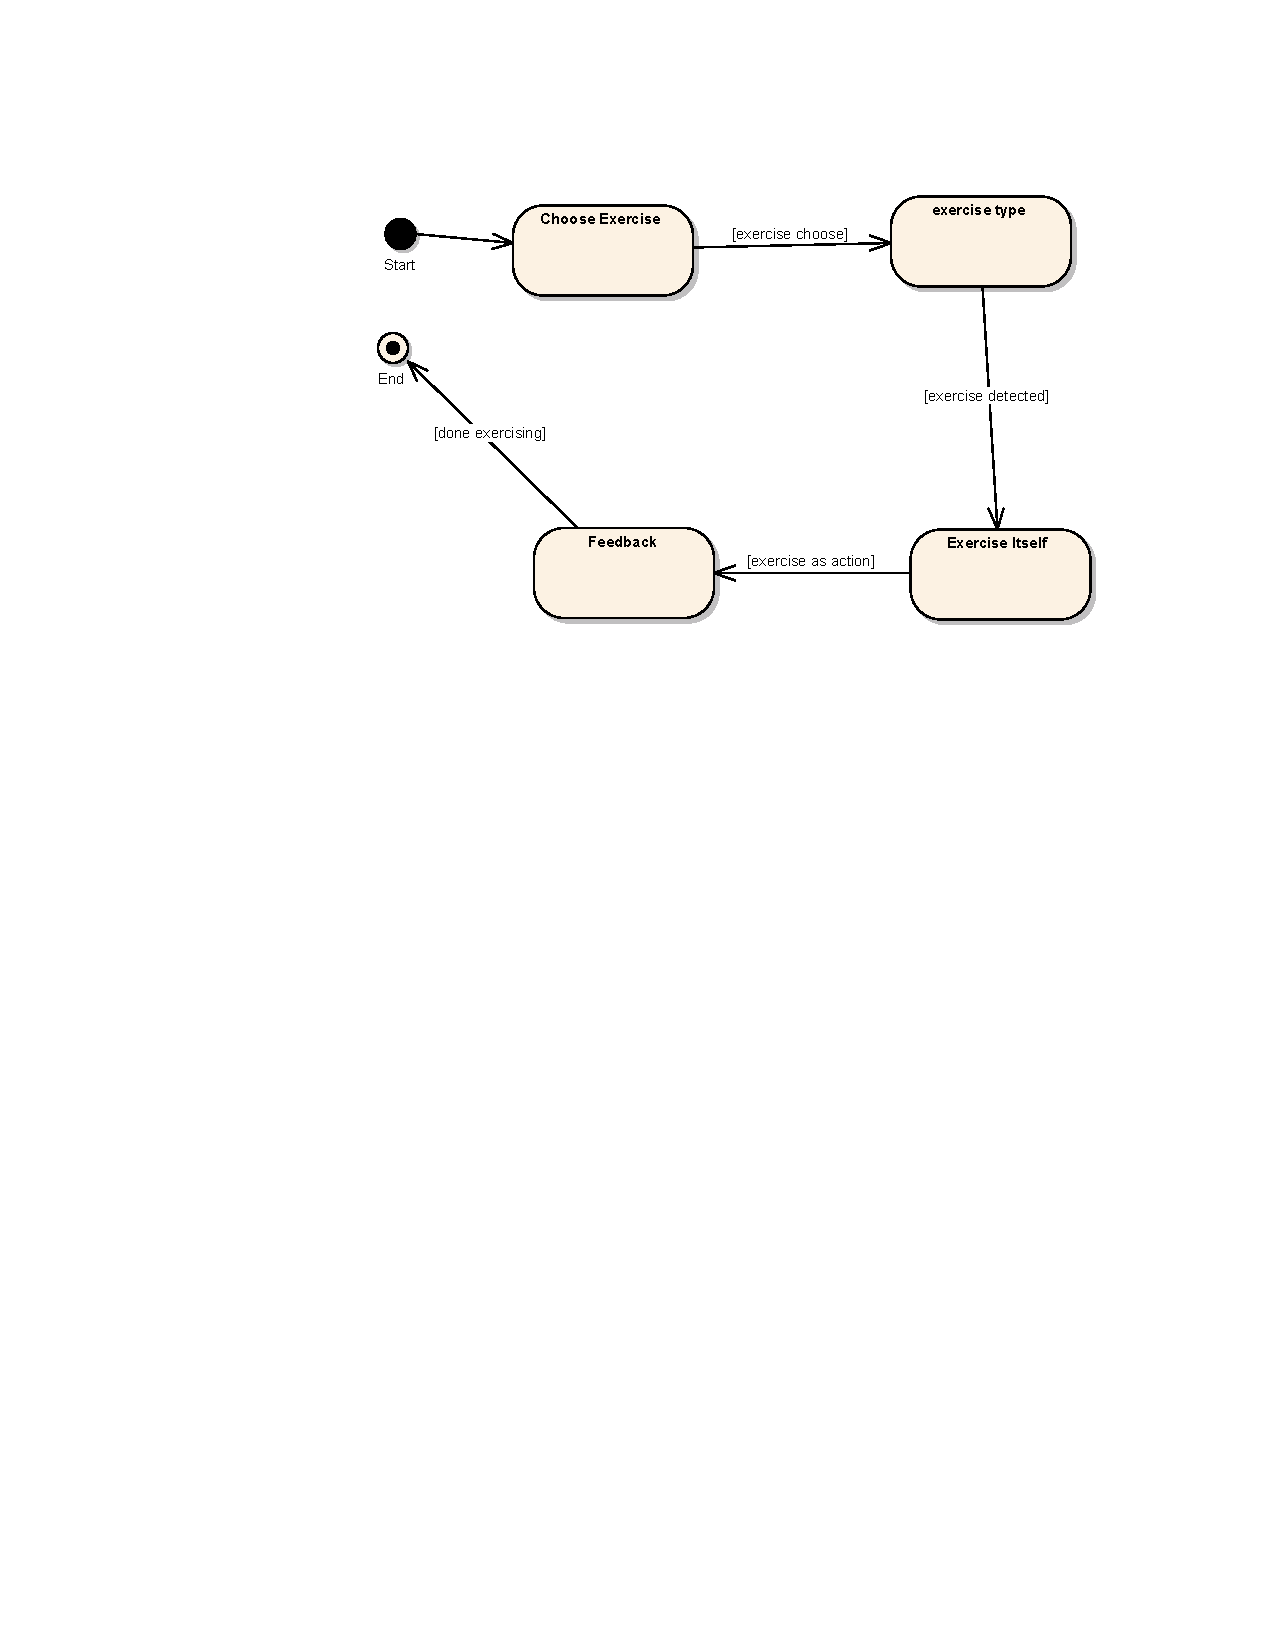
\includegraphics[trim={0 17cm 0 3cm},clip, width = 16cm]{2_state_performexercise}
\caption{State Diagram of exercising step by step.}\label{state_perform}
\end{figure}

\clearpage

\subsection{User Experience}


\clearpage